\section{Results and analysis}\label{sec:results}
\newcommand{\resultspath}{tex/results}

\newcommand{\prlabelplot}[6] {
\addplot+[only marks, fill opacity=0.2,
	discard if not={Method}{#1},
	discard if not={Model}{#2},
	discard if not={Category}{#3},
	discard if not={HistThreshold}{#4},
	discard if not={Label}{#5}
] table [x=Recall, y=Precision, col sep=comma] {\resultspath/kp-labelling.csv};
\addlegendentry{#6}
}


% Tikz graph for labelling
% #1 - Histogram threshold
% #2 - Model used (mature/juvenile)
% #3 - Label
\newcommand{\prlabelgraph}[4]{
\begin{tikzpicture}[scale=0.8]
\begin{axis}[
	title = {\textbf{Histogram threshold of #2}},
	legend pos=outer north east,
	legend entries={
		Graph method on mature lobsters;,
		Label method on mature lobsters;,
		Graph method on juvenile lobsters;,
		Label method on juvenile lobsters
	},
	legend to name=#4,
	xlabel={Recall},
	xmin=0,xmax=1,
	ylabel={Precision},
	ymin=0,ymax=1
]

\prlabelplot{graph}{#1}{mature}{#2}{#3}{Graph method, mature lobsters}
\prlabelplot{model}{#1}{mature}{#2}{#3}{Label method, mature lobsters}
\prlabelplot{graph}{#1}{juvenile}{#2}{#3}{Graph method, juvenile lobsters}
\prlabelplot{model}{#1}{juvenile}{#2}{#3}{Label method, juvenile lobsters}

\end{axis}
\end{tikzpicture}
}


\newcommand{\foneidentplot}[5] {
\addplot+[mark=none,
	discard if not={Method}{#1},
	discard if not={Model}{#2},
	discard if not={Category}{#3},
	discard if not={HistThreshold}{#4}
] table [x=LabelThreshold, y=F1, col sep=comma] {\resultspath/kp-identification.csv};
\addlegendentry{#5}
}

\newcommand{\foneidentgraph}[3]{
\begin{tikzpicture}[scale=0.8]
\begin{axis}[
	title = {\textbf{Histogram threshold of #2}},
	legend pos=outer north east,
	legend entries={
		Graph method on mature lobsters;,
		Label method on mature lobsters;,
		Graph method on juvenile lobsters;,
		Label method on juvenile lobsters
	},
	legend to name=#3,
	xlabel={Label threshold},
	xmin=0,xmax=1,
	xmode=log,
	ylabel={F1 score},
	ymin=0,ymax=1
]

\foneidentplot{graph}{#1}{mature}{#2}{Graph method, mature lobsters}
\foneidentplot{model}{#1}{mature}{#2}{Label method, mature lobsters}
\foneidentplot{graph}{#1}{juvenile}{#2}{Graph method, juvenile lobsters}
\foneidentplot{model}{#1}{juvenile}{#2}{Label method, juvenile lobsters}
\end{axis}
\end{tikzpicture}
}


\newcommand{\fourplotall}[4] {
\begin{minipage}{0.48\textwidth}
	\centering
	#1
\end{minipage}
\hspace*{\fill}
\begin{minipage}{0.48\textwidth}
	\centering
	#2
\end{minipage}
\n
\begin{minipage}{0.48\textwidth}
	\centering
	#3
\end{minipage}
\hspace*{\fill}
\begin{minipage}{0.48\textwidth}
	\centering
	#4
\end{minipage}
}

\newcommand{\fourplot}[3]{
\begin{minipage}{0.48\textwidth}
	\centering
	#1{#2}{0.3}{#3}
\end{minipage}
\hspace*{\fill}
\begin{minipage}{0.48\textwidth}
	\centering
	#1{#2}{0.5}{#3}
\end{minipage}
\n
\begin{minipage}{0.48\textwidth}
	\centering
	#1{#2}{0.7}{#3}
\end{minipage}
\hspace*{\fill}
\begin{minipage}{0.48\textwidth}
	\centering
	#1{#2}{0.9}{#3}
\end{minipage}
}

\newcommand{\fourplotlabel}[4]{
\begin{minipage}{0.48\textwidth}
	\centering
	#1{#2}{0.3}{#3}{#4}
\end{minipage}
\hspace*{\fill}
\begin{minipage}{0.48\textwidth}
	\centering
	#1{#2}{0.5}{#3}{#4}
\end{minipage}
\n
\begin{minipage}{0.48\textwidth}
	\centering
	#1{#2}{0.7}{#3}{#4}
\end{minipage}
\hspace*{\fill}
\begin{minipage}{0.48\textwidth}
	\centering
	#1{#2}{0.9}{#3}{#4}
\end{minipage}
}


The developed models and methods were able to take images from the dataset and to match it with an attributed graph. The graph contains labels for each node that specifies the body part identified and edges that connect each node. Performance of the developed models and methods is then measured to give numeric results. First, a qualitative evaluation on the results of the matched images and graphs was carried out to show the effectiveness of the matching visually. Then a quantitative analysis using different metrics was performed to evaluate how well the methods used in this project is able to perform against previous methods. The quantitative values measured are later compared to Abdallah's results in section \ref{sec:evaluation}. It would be expected for the method developed in this project to give better results. 
\subsection{Experimental design}
For quantifying the results, precision and recall metrics were initially used. The goal of using precision and recall is too see what kind of trade-off there is between the relevant keypoints detected in all detected keypoints (precision) and the relevant keypoints detected in all relevant keypoints (recall). The F1 score was then computed to get the harmonic mean of precision and recall. This allows the best labelling and colour histogram thresholds to be found. Finally, by applying a combination of probability and graph edit distance on the models, images from the rest of the dataset were classified as either mature or juvenile.
\n
They are also two other parameters that were explored in parallel with the evaluation metrics:
\begin{enumerate}
\item As explained in section \ref{sec:graph-creation}, three methods were investigated for rebuilding the matched subgraphs into the final lobster graph. Although the keypoint method was not evaluated due to its shortcomings, the label and graph methods are both used during the evaluation to test which is more effective.
\item In section \ref{sec:annotation}, it was described how the additional annotation of attribute graphs to the lobster images were split into mature and juvenile categories based on the original dataset. The probabilistic models are based on the two sets of annotations and their performance on both mature and juvenile lobsters can be compared. It is also interesting to see if any model performs better with a particular method or for a particular label. 
\end{enumerate}
To calculate the precision and recall, the ground truth of the correct lobster graph must be known and so only the subset of images with annotated attributed graphs are used in precision-recall experiments. 
\n
All measurements needed for evaluation are deterministic, the probabilities and keypoints detected may change based on thresholds, but will not change between runs. As such, only one run of any of the experiments is needed to get the results needed.

\subsection{Qualitative analysis}
A brief qualitative evaluation of the output graph drawn on top of the images is explored here to get a visual glimpse of how the developed algorithm works.
\begin{figure}[H]
	\begin{subfigure}{0.45\textwidth}
	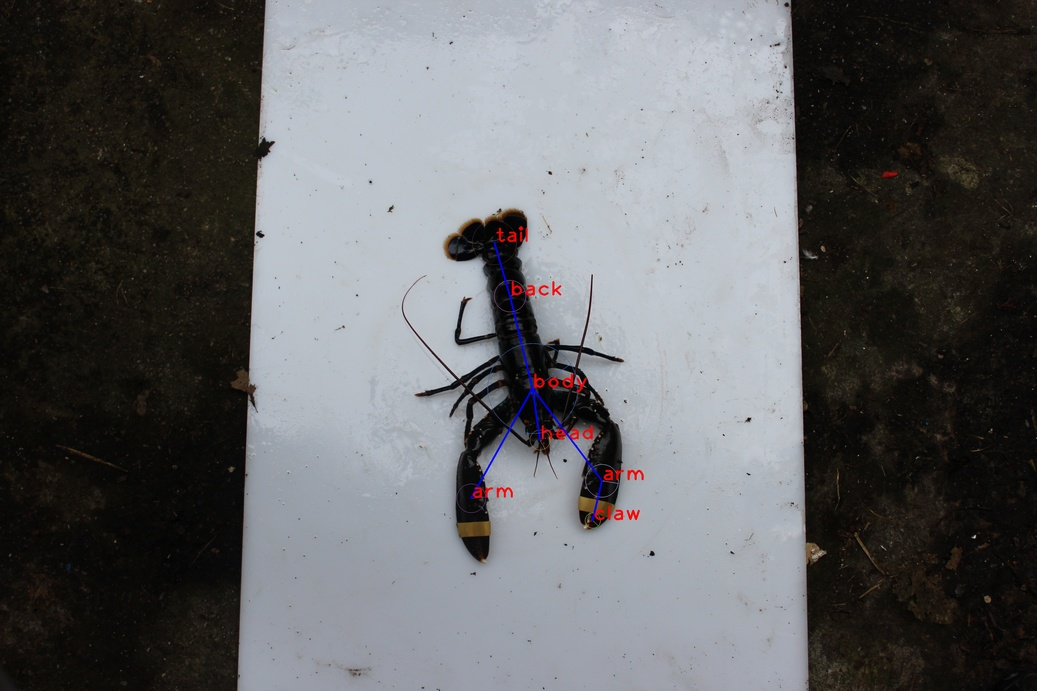
\includegraphics[width=1\textwidth, keepaspectratio]{\resultspath/good-match.JPG}
	\caption{Example of good match}
	\end{subfigure}
	\hspace*{\fill}
	\begin{subfigure}{0.45\textwidth}
	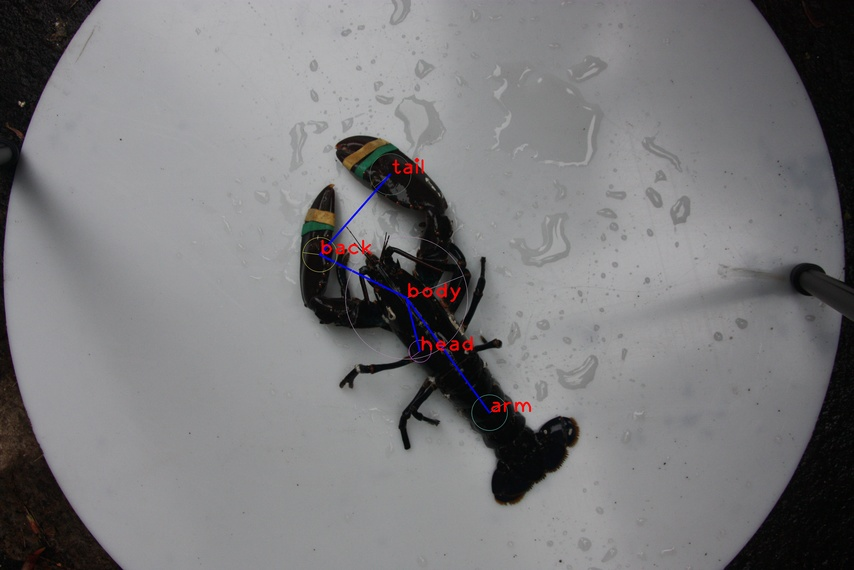
\includegraphics[width=1\textwidth, keepaspectratio]{\resultspath/bad-match.JPG}
	\caption{Example of poor match}
	\label{fig:poor-match}
	\end{subfigure}
\caption{Example of final graph matches. In the case of the poor match, a juvenile model was used on an image of a mature lobster, leading to incorrect labelling despite reasonable keypoint detection.}
\end{figure}
\noindent
It can be seen that when the algorithm works, the graph is matched very well to each body part on the lobster, with the nodes properly connected. Further, the keypoints are all labelled correctly and only one claw keypoint was missing. In the case where the matching was poor, the labels were often incorrect, parts of the graph are missing (no claws) and irrelevant keypoints are detected and labelled. There are three main reasons for this:
\begin{itemize}
\item The keypoint was not detected, so it could not have been matched or labelled
\item Thresholds on labelling and histograms filtered out relevant keypoints
\item Probabilistic model filtered out correct subgraph configurations 
\end{itemize}
Octave filtering is unlikely to remove relevant keypoints because it only removes keypoints that are too small to be suitable. The latter two reasons are more likely than the keypoint not being detected at all because SIFT is able to detect an abundance of keypoints as demonstrated in section \ref{sec:kp-detection}. The other two cases happen more often when the incorrect model is used, for example a juvenile model used on a mature lobster as in figure \ref{fig:poor-match}. The sizes of nodes and lengths of edges are different for the two models and so mislabelling happens more often. Mislabelling can then cause a knock on effect which affects the matching step.

\subsection{Precision and recall}
The evaluation for precision and recall was split into two evaluations, one for the performance of identifying correct keypoints and the second for the performance of keypoint labelling. The evaluations are split into two parts because defining false positives and false negatives when evaluating both aspects together is a difficult problem, the key issue being an overlap between false positives and false negatives for correctly detected but mislabelled keypoints. For example, if a keypoint has been correctly identified and labelled as a \textit{claw} but is actually an \textit{arm}, then it should be a false positive because the labelling is incorrect. However, it should also be a false negative because correct \textit{arm} labelling is missed. Because of these difficult definitions, it made sense to split the precision and recall evaluation into two separate parts where the false positives and false negatives could be clearly defined.
\n
In order to create a precision-recall curve, the probability threshold for labelling keypoints and the threshold for colour histogram filtering is incrementally changed. This shows how the two thresholds affect the precision and recall of the lobster graphs created. Note that results for very low thresholds were not obtained due to the large time taken because of the combinatorial explosion. It would then be expected that as the thresholds changes, the trade-off between precision and recall also changes, for example a high labelling threshold may give lower recall as relevant annotations are missed, but high precision as all keypoints identified in the image are relevant keypoints.

\subsubsection{Keypoint identification}
The precision and recall metrics were calculated for keypoint identification to see how many keypoints from the annotated images could be re-identified in the final graph. The labels of each keypoint and the edges between them were not taken into account for these results. The precision and recall for the evaluation is defined as follows:
\begin{align}
\text{Precision} &= \frac{\text{Correctly detected keypoints}}{\text{Correctly detected keypoints} + \text{Incorrectly detected keypoints}} 
\\[10pt]
\text{Recall} &= \frac{\text{Correctly detected keypoints}}{\text{Correctly detected keypoints} + \text{Missed keypoints in annotation}}
\end{align}
False positives are incorrectly detected keypoints, as they have been identified, but are not correct compared to the truth. The false negatives are keypoints that are in the annotation, but were not detected for the final graph and hence incorrectly identified as an irrelevant keypoint. Keep in mind that the dataset was categorised as either a juvenile or mature lobster and two probability models were created based on the two categories. Both models and categories are tested for results, as it is expected that a mismatch between the two would result in lower performance.
\newcommand{\pridentplot}[5]{
\addplot+[mark=none, fill opacity=0.2, 
	discard if not={Method}{#1}, 
	discard if not={Model}{#2}, 
	discard if not={Category}{#3},
	discard if not={HistThreshold}{#4}
] table [x=Recall, y=Precision, col sep=comma] {\resultspath/kp-identification.csv};
\addlegendentry{#5}
}
% Tikz graph for identification
% #1 - Histogram threshold
% #2 - Model used (mature/junveile)
\newcommand{\pridentgraph}[3]{
\begin{tikzpicture}[scale=0.8]
\begin{axis}[
	title = {\textbf{Histogram threshold of #2}},
	legend pos=south east,
	enlargelimits=true,
	xlabel={Recall},
	xmin=0,xmax=1,
	ylabel={Precision},
	ymin=0,ymax=1
]

\pridentplot{graph}{#1}{mature}{#2}{Graph method, mature lobsters}
\pridentplot{model}{#1}{mature}{#2}{Label method, mature lobsters}
\pridentplot{graph}{#1}{juvenile}{#2}{Graph method, juvenile lobsters}
\pridentplot{model}{#1}{juvenile}{#2}{Label method, juvenile lobsters}

\end{axis}
\end{tikzpicture}
}


\begin{figure}[H]
\centering
\fourplot{\pridentgraph}{mature}{legend:prident}
\caption{Precision/recall graphs using the mature model with varying label thresholds.}
\label{fig:pridentmat}
\end{figure}

\begin{figure}[H]
\centering
\fourplot{\pridentgraph}{juvenile}{legend:prident}
\caption{Precision/recall graphs using the juvenile model with varying label thresholds.}
\label{fig:pridentjuv}
\end{figure}
\noindent
It can be seen from figure \ref{fig:pridentjuv} and \ref{fig:pridentmat} that despite the variation of the label and histogram thresholds, there is not a clear precision-recall curve that shows the trade-off between the two metrics. The change in the labelling threshold clearly affects the recall, but precision seems independent of both the recall and thresholds as it says relatively the same even though recall improves dramatically. This suggests there is either no inherent trade-off between precision and recall in this problem, or the thresholds being changed is not suitable to find the trade-off and therefore does not affect it. 
\n
The varying label and histogram filtering thresholds may not have provided useful functions as they only indirectly affect the final graph that is built. The two thresholds significantly change what labels and keypoints are kept in the stages leading up to the creation of the final graph, for example a high label threshold would mean less subgraphs to explore as less labels could be applied. However it is the probabilistic model of choosing subgraphs which ultimately affects the lobster graph that is created. The issue here is that there is no threshold that can be applied to this probabilistic model, as the most probable subgraphs are chosen incrementally. For this reason, examining the precision and recall metrics is not suitable to evaluate performance. 
\n
Another interesting thing to note here is the difference between using a mature lobster model (figure \ref{fig:pridentmat}) and using a juvenile lobster model (figure \ref{fig:pridentjuv}). There is a clear difference in both precision and recall when applying the juvenile model to the two categories of images. However, the difference is less obvious with the mature model. The smaller difference may come from the increased variance in the mature lobster images for sizes of keypoints and length of edges. On the other hand, the juvenile lobster images are more consistent with the lobster sizes. 

\subsubsection{Keypoint labelling}
In the evaluation of keypoint labelling, the precision-recall calculations are altered slightly because only the labels on the detected keypoints matter here, rather than the detection itself. Additionally, the evaluation can be focused on each specific label (claw, tail, etc.) to see if there are any strengths of weaknesses for specific body parts. Precision and recall for here are defined as follows:
\begin{align}
\text{Precision} &= \frac{\text{Correctly labelled keypoints}}{\text{Correctly labelled keypoints} + \text{Incorrectly labelled keypoints}}
\\[10pt]
\text{Recall} &= \frac{\text{Correctly labelled keypoints}}{\text{Correctly labelled keypoints} + \text{Missed labels in annotation}}
\end{align}
Incorrectly labelled keypoints are either ones where the keypoint was wrong, in which case the label is incorrect by default, or the keypoint is correct, but the label is wrong compared to the annotations. These are classified as false positives. The false negatives are labels which were missed in the annotations, for example if there were two claw labels in the annotations but only one claw was found in the final graph. 

\begin{figure}[H]
\centering
\fourplotlabel{\prlabelgraph}{mature}{claw}{legend:prlabel}
\ref{legend:prlabel}
\caption{Precision/recall graphs with the mature model for label \textit{claw}.}
\end{figure}

\begin{figure}[H]
\centering
\fourplotlabel{\prlabelgraph}{juvenile}{claw}{legend:prlabel}
\ref{legend:prlabel}
\caption{Precision/recall graphs with the juvenile model for label \textit{claw}. Further graphs of all other labels can be found in appendix TODO}
\end{figure}
\noindent
The precision-recall graphs for labels confirm that precision and recall are not very suitable metrics due to the lack of a good threshold to alter. There seems to be something missing in the curves, as the linear relationship from varying label thresholds and different methods and models is not expected from a precision-recall curve. Potentially each point in the graphs represent a separate precision-recall curve, but the threshold required to be varied that gives the trade-off and the rest of the curve could not be found.
%
%\begin{figure}[H]
%\centering
%\fourplotlabel{\prlabelgraph}{juvenile}{arm}{legend:prlabel}
%\ref{legend:prlabel}
%\caption{Precision/recall with juvenile model for label ``arm"}
%\end{figure}
%
%\begin{figure}[H]
%\centering
%\fourplotlabel{\prlabelgraph}{juvenile}{tail}{legend:prlabel}
%\ref{legend:prlabel}
%\caption{Precision/recall with juvenile model for label ``tail"}
%\end{figure}
%
%\begin{figure}[H]
%\centering
%\fourplotlabel{\prlabelgraph}{juvenile}{tail}{legend:prlabel}
%\ref{legend:prlabel}
%\caption{Precision/recall with juvenile model for label ``head"}
%\end{figure}


\subsection{F1 score}
Although precision and recall did not give much insight into the models and methods used, the metrics can still be used to empirically find the best labelling and histogram filtering thresholds that should be used for classification. The F1 score can be used as a weighted average of precision and recall where both contribute equally. The scores ranges from 0 to 1, where 1 means perfect precision and recall. The best thresholds are therefore those whose F1 score is the highest. The F1 score also gives a reasonable look into which models and methods are the most effective. The identification and labelling evaluations continue to be kept separate for the same reason as mentioned above. 
\subsubsection{Keypoint identification}

\begin{figure}[H]
\centering
\fourplot{\foneidentgraph}{mature}{legend:foneident}
\\
\ref{legend:foneident}
\caption{F1 score for varying thresholds with the mature model.}
\label{fig:fonemature}
\end{figure}

\begin{figure}[H]
\centering
\fourplot{\foneidentgraph}{juvenile}{legend:foneident}
\\
\ref{legend:foneident}
\caption{F1 score for varying thresholds with the juvenile model.}
\label{fig:fonejuvenile}
\end{figure}

\begin{table}[H]
\centering
\begin{tabular}{| c | c | c | c | c | c |}
\hline
\textbf{Method} & \textbf{Model} & \textbf{Category} & \textbf{Label threshold} & \textbf{Histogram threshold} & \textbf{F1 score} \\ 
\hline
Graph & Juvenile & Juvenile & 0.03 & 0.3-0.9 & 0.880 \\
\hline
Label & Juvenile & Juvenile & 0.03 & 0.3-0.7 & 0.844 \\
\hline
Label & Mature & Juvenile & 0.07 & 0.5-0.7 & 0.765 \\
\hline
Label & Mature & Mature & 0.05 & 0.3 & 0.726 \\
\hline
Graph & Mature & Juvenile & 0.08 & 0.5-0.7 & 0.718 \\
\hline
Graph & Mature & Mature & 0.06-0.05 & 0.3 & 0.694 \\
\hline
Label & Juvenile & Mature & 0.03 & 0.3-0.7 & 0.487 \\
\hline
Graph & Juvenile & Mature & 0.05 & 0.3-0.7 & 0.434 \\
\hline
\end{tabular}
\caption{Best F1 score and thresholds for different combinations of methods and models.}
\end{table}
\noindent
In general, it is shown clearly that the label threshold has a substantial impact on performance. As the label threshold increases, the F1 score decreases because it becomes less probable for any particular label to be applied to a keypoint. The decreased number of labelled keypoints then cause less subgraphs to be matched and so reduces the number of final keypoints. Moreover, at high label thresholds, it becomes more likely that a keypoint will not be labelled at all and so additional relevant information is lost. 
\n
The histogram threshold seems to have less of an impact as little difference can be seen between each graph with a different histogram threshold. This is interesting because with a low histogram threshold, more irrelevant keypoints will be kept so it would be expected that the F1 score decreases. The lack of an impact by the histogram threshold has two possible explanations which are not mutually exclusive:
\begin{enumerate}
\item The colour histogram filtering is very effective such that irrelevant keypoints require a very low threshold to be included. 
\item The probabilistic models are effective in removing irrelevant keypoints, so the resulting lobster graphs are still the same or very similar even when more keypoints are introduced. 
\end{enumerate}
Of the two explanations, the latter seems more possible. As demonstrated in section \ref{sec:colour-histogram}, a colour histogram filter can still result in irrelevant keypoints being detected. As such, the lower threshold likely adds more keypoints to be matched, but the matching steps and the building of further probabilistic graphs are robust against such noise, which is why little difference can be seen between the different histogram thresholds. 
\n
The graphs of figure \ref{fig:fonemature} and \ref{fig:fonejuvenile} further demonstrate juvenile lobsters being better detected in general, regardless of the model or method used, when compared to mature lobsters. 
\subsubsection{Keypoint labelling}
The F1 score is also looked into for the labelling to see if any particular labels perform better. This would be interesting to see if certain labels are detected with higher certainty compared to others, showing the strengths and weaknesses for each method and model.

\begin{table}[H]
\centering
\begin{tabular}{| c | c |}
\hline
\textbf{Label} & \textbf{F1 score} \\
\hline
Body & 0.99 \\
Tail & 0.70 \\
Head & 0.58 \\
Arm & 0.57 \\
Claw & 0.45 \\
Back & 0.34 \\
\hline
\end{tabular}
\caption{Average F1 score for each label, averaged over all over parameters}
\label{tbl:avg-allf1}
\end{table}
\noindent
The average F1 score for all labels can be seen in table \ref{tbl:avg-allf1}. The average is used to show which labels can be detected and labelled correctly the most regardless of the methods or thresholds. The body keypoint is found very reliably, almost 100\% of the time. Because subgraphs of 3 nodes were chosen as the intermediate between matching and rebuilding the complete graph, finding the body keypoints is very important as every 3 node subgraph must contain a body. In cases where the body is not detected, no final graph can be created as no subgraphs will be matched.
\n
The tail label can also be found reasonably and this can be expected as it is a very distinct feature on the lobster. The ability to discover the tail node is key for tail width measurement, which can be important depending on what features of the lobster need to be measured. Interestingly, the arms and claws are not as easily found despite also being distinct features. This could be due to other irrelevant keypoints found on the lobster that match the same size and distance of the claws and arms to the body, causing incorrect matches. 

\begin{table}[H]
\centering
\begin{tabular}{| c | c | c | c |}
\hline
\textbf{Label} & \textbf{F1 score} & \textbf{Label threshold} & \textbf{Histogram threshold} \\
\hline
Body & 1.0 & 0.3-0.1 & 0.3-0.9 \\
Tail & 0.94 & 0.35 & 0.3-0.9 \\
Head & 0.75 & 0.55 & 0.9 \\
Arm & 0.66 & 0.6 & 0.3 \\
Back & 0.5 & 0.27-0.29 & 0.3-0.9 \\
Claw & 0.49 & 0.45 & 0.3 \\
\hline
\end{tabular}
\caption{Best F1 score for each label, averaged over all methods, models and categories to show the best thresholds that can be used for each label.}
\label{tbl:avg-f1}
\end{table}

 
\newcommand{\fonelabelplot}[6] {
\addplot+[mark=none,
	discard if not={Method}{#1},
	discard if not={Model}{#2},
	discard if not={Category}{#3},
	discard if not={HistThreshold}{#4},
	discard if not={Label}{#5}
] table [x=LabelThreshold, y=F1, col sep=comma] {\resultspath/kp-labelling.csv};
\addlegendentry{#6}
}

\newcommand{\fonelabelgraph}[4]{
\begin{tikzpicture}[scale=0.75]
\begin{axis}[
	title = {\textbf{Histogram threshold of #2}},
	legend pos=outer north east,
	legend entries={
		Graph method on mature lobsters;,
		Label method on mature lobsters;,
		Graph method on juvenile lobsters;,
		Label method on juvenile lobsters
	},
	legend to name=#4,
	xlabel={Label threshold},
	xmin=0,xmax=1,
	%xmode=log,
	ylabel={F1 score},
	ymin=0,ymax=1
]

\fonelabelplot{graph}{#1}{mature}{#2}{#3}{Graph method on mature lobsters}
\fonelabelplot{model}{#1}{mature}{#2}{#3}{Label method on mature lobsters}
\fonelabelplot{graph}{#1}{juvenile}{#2}{#3}{Graph method on juvenile lobsters}
\fonelabelplot{model}{#1}{juvenile}{#2}{#3}{Label method on juvenile lobsters}
\end{axis}
\end{tikzpicture}
}

\begin{figure}[H]
\centering
\fourplotlabel{\fonelabelgraph}{juvenile}{arm}{legend:fone-label}
\ref{legend:fone-label}
\caption{Juvenile lobster model on the arm label}
\label{fig:fone-juv-arm}
\end{figure}

\begin{figure}[H]
\centering
\fourplotlabel{\fonelabelgraph}{juvenile}{head}{legend:fone-label}
\ref{legend:fone-label}
\caption{Juvenile model, head label}
\label{fig:fone-juv-head}
\end{figure}
\noindent
The range of thresholds shown in table \ref{tbl:avg-f1} and the varying performance of different methods shown in figures \ref{fig:fone-juv-arm} and \ref{fig:fone-juv-head} indicates that different labels are affected by different thresholds and methods. For example, the model used for the arm label has little effect on its F1 score as there is lots of overlap between the mature and juvenile models. However, the model used for the head label has a much larger effect, where the correct model (juvenile model on juvenile lobster) massively outperforms itself against incorrect lobster categories. Further, unlike the F1 scores for keypoint identification, it is not clear that lowering the label threshold lowers the score. The complicated issue with the combination of all the different parameters is interesting for further exploration, especially for labels with lower average F1 score such as the claw or arm. 



\subsection{Classification}
As both a mature and juvenile model are developed to match to the lobster images, how well each model is matched to the lobster in the image can be used for classification. For example, if the image contains a mature lobster, then the mature model would be expected to be better matched compared to the juvenile model. 
\n
As a probabilistic model was developed and used for the creation and matching steps to produce the final matched lobster graph, the use of probabilities is again explored for classification. To use probabilities for classification, the product of the probabilities for each node and edge can be calculated as was done in section \ref{sec:graph-creation}. This would give two probabilities, one for each graph created by the mature and juvenile models. However, in cases where nodes and edges were not identified, the probability of the graph would increase because the probabilities are multiplied. This is the opposite of what is desired, as missing nodes and edges should incur heavy penalties. Furthermore, there is no easy way give a penalty to missing nodes and edges without being too arbitrary. Therefore, using just the probabilities is not a very suitable way to define the two classifications.
\n
With the two final graphs of mature and juvenile lobsters, a graph similarity score can be computed. The graph edit distance is typically used as a distance measure between two graphs. It is defined as the weighted sum of the cost of edits such as node insertion or edge deletion required to convert one graph to the other. The maximum common subgraph as described in section \ref{sec:lit-graph} is another concept that can be applied. The larger the maximum common subgraph between the matched graph and ideal graph, the better the match. There are a variety of such algorithms for graph similarity and matching that could be further explored \cite{graph-similarity}. In \cite{graph-edit}, Bunke proved that by using a particular cost function, the computation for the graph edit distance is equivalent to the maximum common subgraph problem. The problem with using edit distance metrics is that it does not take into account errors in labelling and matching. In other words, a matched lobster graph can have a very small distance metric to the ideal lobster graph because most of the body parts and edges were identified, however the body parts could be mislabelled and the edit distance would not be able to allow for this issue. 
\n
As such, a combination of the probability and graph edit distance must be used to determine how well a detected graph matches to an ideal graph to classify images without ground truths. 

\subsubsection{Validation}

From the results of precision, recall and F1 score, it was shown that there was a much clearer performance difference applying the juvenile model to mature and juvenile lobsters. Further, juvenile lobsters still had high F1 scores even when applied to mature lobsters. For this reason, the classification results TODO.
\n
To show why graph edit distance alone is not strong enough a metric for classification, a validation test with the annotated dataset is run. The classification is determined by calculating the edit distance from the matched lobster graph and the ideal lobster graph where all body parts are found and identified. The cost functions for the edit distance are defined following Bunke's paper \cite{graph-edit}. Both mature and juvenile models are used and the model with the lower edit distance is chosen as the classification. It is unclassified if the two edit distances are equal. 
\begin{figure}[H]
\centering
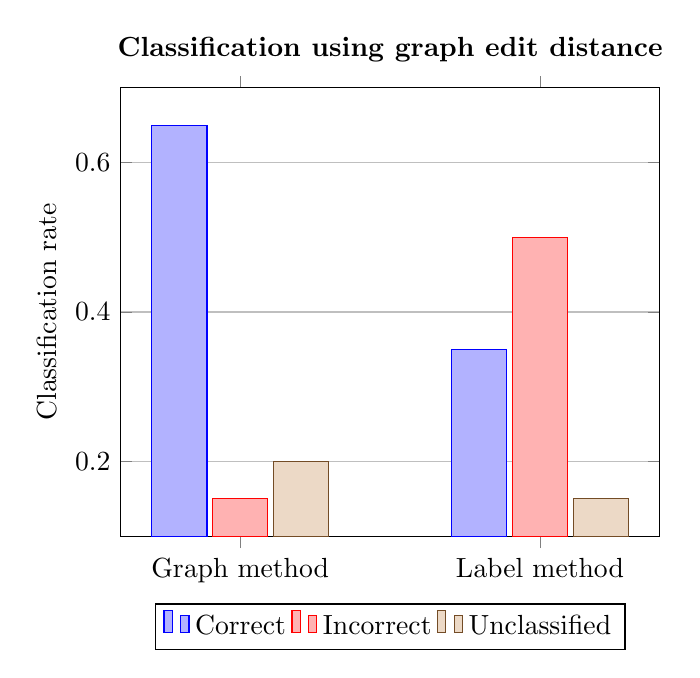
\begin{tikzpicture}
\begin{axis}[
    ybar,
    title={\textbf{Classification using graph edit distance}},
    bar width=2em,
    enlarge x limits=0.4,
    legend style={
      at={(0.5,-0.15)},
      anchor=north,legend columns=-1
    },
    ylabel={Classification rate},
    symbolic x coords={Graph method,Label method},
    xtick=data,
    ymajorgrids=true, 
]
\addplot coordinates {(Graph method, 0.65) (Label method, 0.35)};
\addlegendentry{Correct}

\addplot coordinates {(Graph method, 0.15) (Label method, 0.5)};
\addlegendentry{Incorrect}

\addplot coordinates {(Graph method, 0.2) (Label method, 0.15)};
\addlegendentry{Unclassified}
\end{axis}
\end{tikzpicture}
\caption{Overall classification rate for using graph edit distance to determine classification}
\end{figure}
\noindent

\begin{figure}[H]
\centering
\begin{minipage}{0.48\textwidth}
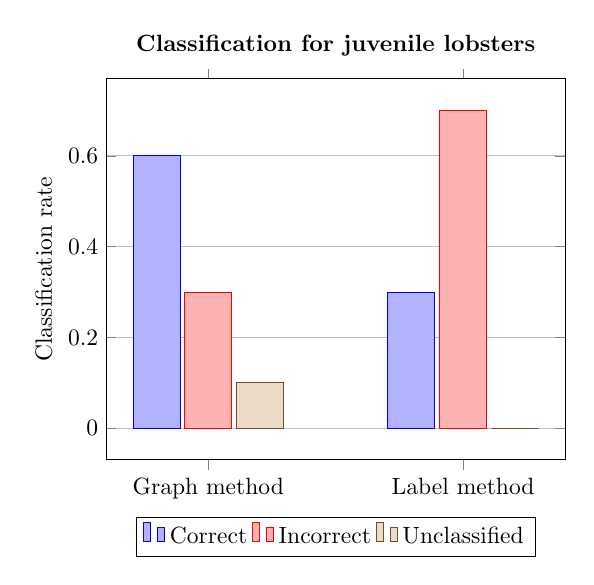
\begin{tikzpicture}[scale=0.85]
\begin{axis}[
    ybar,
    title={\textbf{Classification for juvenile lobsters}},
    bar width=2em,
    enlarge x limits=0.4,
    legend style={
      at={(0.5,-0.15)},
      anchor=north,legend columns=-1
    },
    ylabel={Classification rate},
    symbolic x coords={Graph method,Label method},
    xtick=data,
    ymajorgrids=true, 
]
\addplot coordinates {(Graph method, 0.6) (Label method, 0.3)};
\addlegendentry{Correct}

\addplot coordinates {(Graph method, 0.3) (Label method, 0.7)};
\addlegendentry{Incorrect}

\addplot coordinates {(Graph method, 0.1) (Label method, 0)};
\addlegendentry{Unclassified}
\end{axis}
\end{tikzpicture}
\end{minipage}
\hspace*{\fill}
\begin{minipage}{0.48\textwidth}
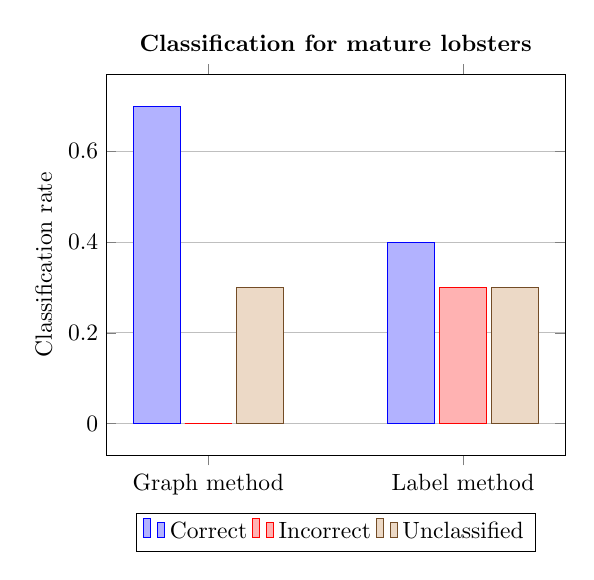
\begin{tikzpicture}[scale=0.85]
\begin{axis}[
    ybar,
    title={\textbf{Classification for mature lobsters}},
    bar width=2em,
    enlarge x limits=0.4,
    legend style={
      at={(0.5,-0.15)},
      anchor=north,legend columns=-1
    },
    ylabel={Classification rate},
    symbolic x coords={Graph method,Label method},
    xtick=data,
    ymajorgrids=true, 
]
\addplot coordinates {(Graph method, 0.7) (Label method, 0.4)};
\addlegendentry{Correct}

\addplot coordinates {(Graph method, 0) (Label method, 0.3)};
\addlegendentry{Incorrect}

\addplot coordinates {(Graph method, 0.3) (Label method, 0.3)};
\addlegendentry{Unclassified}
\end{axis}
\end{tikzpicture}
\end{minipage}
\caption{More detailed classification results on the specific lobster categories.}
\end{figure}




%\subsection{Testing the models}


